\documentclass[12pt,a4paper]{article}

% --- Page Layout -------------------------------------------------------------
\usepackage[a4paper, margin=0.8in, headheight=14pt]{geometry}

% --- Fonts (XeLaTeX) ---------------------------------------------------------
\usepackage{fontspec}
\usepackage{unicode-math}
\setmainfont{TeX Gyre Pagella}
\setmonofont[Scale=0.88]{TeX Gyre Cursor}
\setmathfont{Latin Modern Math}

% --- Packages ---------------------------------------------------------------
\usepackage{xcolor}
\usepackage{titlesec}
\usepackage{enumitem}
\usepackage{tabularx}
\usepackage{booktabs}
\usepackage{array}
\usepackage{amsmath}
\usepackage{tikz}
\usetikzlibrary{shapes.geometric, arrows.meta, positioning, calc, fit, decorations.pathreplacing, decorations.pathmorphing}
\usepackage{tcolorbox}
\tcbuselibrary{skins, breakable}
\usepackage{hyperref}
\usepackage{fancyhdr}
\usepackage{graphicx}
\usepackage{microtype}
\hyphenpenalty=10000
\exhyphenpenalty=10000
\sloppy
\usepackage{caption}
\usepackage{setspace}
\usepackage{multirow}
\usepackage{tocloft}

% --- Q&A helper --------------------------------------------------------------
\newcommand{\Q}[1]{\textbf{#1}\par\noindent\ignorespaces}

% --- Colour Palette ----------------------------------------------------------
\definecolor{myred}{RGB}{196,30,58}
\definecolor{mydark}{RGB}{30,30,50}
\definecolor{mygreen}{RGB}{14,120,80}
\definecolor{myteal}{RGB}{0,130,140}
\definecolor{myamber}{RGB}{180,100,0}
\definecolor{mypurple}{RGB}{100,30,160}
\definecolor{mygray}{RGB}{246,247,249}
\definecolor{mgframe}{RGB}{180,185,200}
\definecolor{watermark}{RGB}{145,150,170}
\definecolor{hdrred}{RGB}{250,232,235}
\definecolor{hdrgreen}{RGB}{220,244,233}
\definecolor{hdrteal}{RGB}{220,242,244}
\definecolor{hdramber}{RGB}{253,242,215}
\definecolor{hdrpurple}{RGB}{238,228,255}

% --- Section Formatting ------------------------------------------------------
\titleformat{\section}
  {\large\bfseries\color{myred}}{\thesection.}{0.5em}{}
  [\vspace{1pt}{\color{myred}\rule{\linewidth}{0.8pt}}]
\titleformat{\subsection}
  {\normalsize\bfseries\color{myteal}}{\thesubsection}{0.5em}{}
\titlespacing*{\section}{0pt}{18pt}{7pt}
\titlespacing*{\subsection}{0pt}{11pt}{4pt}

% --- Paragraph ---------------------------------------------------------------
\setlength{\parindent}{0pt}
\setlength{\parskip}{4pt}

% --- TOC Styling -------------------------------------------------------------
\renewcommand{\cfttoctitlefont}{\large\bfseries\color{myred}}
\renewcommand{\cftaftertoctitle}{\par\noindent{\color{myred}\rule{\linewidth}{0.8pt}}}
\setlength{\cftbeforetoctitleskip}{0pt}
\setlength{\cftaftertoctitleskip}{6pt}
\renewcommand{\cftsecfont}{\normalsize\bfseries\color{mydark}}
\renewcommand{\cftsecpagefont}{\normalsize\bfseries\color{mydark}}
\renewcommand{\cftsecleader}{\cftdotfill{\cftdotsep}}
\setlength{\cftbeforesecskip}{7pt}
\renewcommand{\cftsubsecfont}{\small\color{mydark}}
\renewcommand{\cftsubsecpagefont}{\small\color{mydark}}
\setlength{\cftbeforesubsecskip}{3pt}
\setlength{\cftsubsecindent}{1.4em}

% --- Table helpers -----------------------------------------------------------
\renewcommand{\arraystretch}{1.45}
\setlength{\tabcolsep}{6pt}
\newcolumntype{B}[1]{>{\small\bfseries\raggedright\arraybackslash}m{#1}}
\newcolumntype{Y}{>{\small\raggedright\arraybackslash}X}
\renewcommand{\tabularxcolumn}[1]{m{#1}}

% --- Header / Footer ---------------------------------------------------------
\pagestyle{fancy}
\fancyhf{}
\fancyhead[L]{\small\color{myred}\textbf{BS-PH101}\;\color{mydark}--- Physics-I}
\fancyhead[R]{\small\color{myteal}\textbf{Module 1 Notes}}
\fancyfoot[C]{\small\color{mydark}\thepage}
\fancyfoot[R]{\small\color{watermark}\textit{\copyright\ Biraj}}
\renewcommand{\headrulewidth}{0.5pt}
\renewcommand{\footrulewidth}{0.3pt}

% --- Hyperref ---------------------------------------------------------------
\hypersetup{
  colorlinks=true, linkcolor=myteal, urlcolor=myteal,
  pdfauthor={Biraj Sarkar},
  pdftitle={BS-PH101 --- Module 1 Notes}
}

% --- tcolorbox styles --------------------------------------------------------
\tcbset{
  tikzbox/.style={
    colback=mygray, colframe=mgframe, boxrule=0.6pt, arc=4pt,
    left=8pt, right=8pt, top=6pt, bottom=6pt,
    colbacktitle=mgframe, coltitle=mydark, fonttitle=\small\bfseries
  },
  defbox/.style={
    colback=hdrgreen, colframe=mygreen, boxrule=0.8pt, arc=4pt,
    left=9pt, right=9pt, top=6pt, bottom=6pt,
    colbacktitle=mygreen, coltitle=white, fonttitle=\small\bfseries
  },
  formulabox/.style={
    colback=hdrteal, colframe=myteal, boxrule=0.8pt, arc=4pt,
    left=9pt, right=9pt, top=7pt, bottom=7pt,
    colbacktitle=myteal, coltitle=white, fonttitle=\small\bfseries
  },
  examplebox/.style={
    colback=hdramber, colframe=myamber, boxrule=0.8pt, arc=4pt,
    left=9pt, right=9pt, top=6pt, bottom=6pt,
    colbacktitle=myamber, coltitle=white, fonttitle=\small\bfseries
  },
  masonbox/.style={
    colback=hdrpurple, colframe=mypurple, boxrule=0.8pt, arc=4pt,
    left=9pt, right=9pt, top=6pt, bottom=6pt,
    colbacktitle=mypurple, coltitle=white, fonttitle=\small\bfseries
  },
  exambox/.style={
    colback=hdrpurple, colframe=mypurple, boxrule=1pt, arc=5pt,
    left=10pt, right=10pt, top=8pt, bottom=8pt,
    colbacktitle=mypurple, coltitle=white, fonttitle=\bfseries,
    breakable, title after break={\textbf{Frequently Asked / Viva Questions (contd.)}}
  }
}
\tcbset{breakable}

% --- TikZ Styles -------------------------------------------------------------
\tikzset{
  block/.style={rectangle, draw=myteal, fill=hdrteal, text width=2.4cm, align=center, minimum height=0.95cm, font=\small, rounded corners=3pt, line width=0.7pt},
  redblock/.style={rectangle, draw=myred, fill=hdrred, text width=2.4cm, align=center, minimum height=0.95cm, font=\small, rounded corners=3pt, line width=0.7pt},
  arrow/.style={-Stealth, thick, color=mydark},
  redarrow/.style={-Stealth, thick, color=myred},
  line/.style={thick, color=mydark}
}

\begin{document}

% --- Title Page --------------------------------------------------------------
\begin{center}
  {\LARGE\bfseries\color{myred} BS-PH101 --- Physics-I}\\[5pt]
  {\normalsize\color{mydark} Semester I/II \quad$\bullet$\quad 3L:1T:0P \quad$\bullet$\quad 4 Credits}\\[3pt]
  {\normalsize\color{myteal}\textbf{Module 1 Comprehensive Exam Notes: Mechanics}}\\[3pt]
  {\small\color{mydark} CGEC \;$|$\; B.Tech ECE (2023--27) \;$|$\; \textit{Biraj Sarkar}}
\end{center}
\vspace{2pt}
\noindent{\color{myred}\rule{\linewidth}{1.5pt}}
\vspace{2pt}
\hypersetup{linkcolor=mydark}
\tableofcontents
\hypersetup{linkcolor=myteal}
\newpage

% =============================================================================
% SECTION 1: CONSTRAINTS & FRICTION
% =============================================================================
\section{Constraints and Friction}

\subsection{Constraints and Degrees of Freedom}

\begin{tcolorbox}[defbox, title={\textbf{Definition: Constraint and Degrees of Freedom}}]
A \textbf{constraint} is any physical restriction on the position or motion of a mechanical system. The number of independent coordinates required to completely specify the configuration of a system is called its \textbf{Degrees of Freedom (DOF)}.
\end{tcolorbox}

If a system consists of $N$ particles in 3D space subject to $k$ independent constraint equations, the number of degrees of freedom is given by:
\begin{equation}
f = 3N - k
\end{equation}

\textbf{Classification of Constraints:}\par\vspace{6pt}\noindent
\begin{tabularx}{\linewidth}{|B{3.2cm}|Y|Y|}
\hline
\textbf{Constraint Type} & \textbf{Condition / Mathematical Form} & \textbf{Physical Example} \\
\hline
\textbf{Holonomic} & Expressible as $f(r_1, r_2, \ldots, r_N, t) = 0$ (integrable algebraic relations). & Rigid body ($|\vec{r}_i - \vec{r}_j| = c$), simple pendulum ($r = L$). \\
\hline
\textbf{Non-Holonomic} & Expressible as inequalities or non-integrable differential relations ($f(\vec{r}, \dot{\vec{r}}, t) = 0$). & Rolling without slipping on a rough plane, gas molecules in a container ($r \le R$). \\
\hline
\textbf{Scleronomic} & Constraint equations do not explicitly depend on time $t$ ($\partial f / \partial t = 0$). & Bead on a fixed wire ring, rigid dumbbell. \\
\hline
\textbf{Rheonomic} & Constraint equations explicitly depend on time $t$ ($\partial f / \partial t \neq 0$). & Bead on a wire ring rotating with constant angular velocity $\omega$. \\
\hline
\end{tabularx}

\subsection{Friction and Laws of Friction}

Friction is the resistive contact force that opposes the relative motion or tendency of relative motion between two surfaces in contact.

\begin{tcolorbox}[formulabox, title={\textbf{Key Laws and Relations of Friction}}]
\begin{itemize}[leftmargin=*, itemsep=2pt]
  \item \textbf{Static Friction ($f_s$):} Self-adjusting force. Maximum value is limiting friction:
  \begin{equation}
  f_{s,\max} = \mu_s N
  \end{equation}
  \item \textbf{Kinetic Friction ($f_k$):} Constant resistive force during motion:
  \begin{equation}
  f_k = \mu_k N \quad (\text{where } \mu_k < \mu_s)
  \end{equation}
  \item \textbf{Angle of Friction ($\lambda$):} Angle between total contact reaction $\vec{R}$ and normal reaction $\vec{N}$:
  \begin{equation}
  \tan \lambda = \frac{f_{s,\max}}{N} = \mu_s \implies \lambda = \tan^{-1}(\mu_s)
  \end{equation}
  \item \textbf{Angle of Repose ($\theta_r$):} Maximum angle of inclination of a rough plane at which a body remains at rest without sliding:
  \begin{equation}
  m g \sin \theta_r = \mu_s m g \cos \theta_r \implies \tan \theta_r = \mu_s \implies \theta_r = \lambda
  \end{equation}
\end{itemize}
\end{tcolorbox}

\begin{tcolorbox}[examplebox, title={\textbf{Solved Problem 1: Block on an Inclined Plane with Friction}}]
\textbf{Problem:} A block of mass $m = 5\text{ kg}$ rests on an inclined plane of angle $\theta = 30^\circ$. The coefficient of static friction is $\mu_s = 0.4$. Determine whether the block slides down, and find the frictional force.

\textbf{Solution:}\par\noindent
\begin{enumerate}[leftmargin=*, itemsep=2pt]
  \item Component of gravity along the incline: $F_{\text{down}} = m g \sin 30^\circ = 5 \times 9.8 \times 0.5 = 24.5\text{ N}$.
  \item Normal reaction: $N = m g \cos 30^\circ = 5 \times 9.8 \times 0.866 = 42.435\text{ N}$.
  \item Maximum limiting static friction: $f_{s,\max} = \mu_s N = 0.4 \times 42.435 = 16.97\text{ N}$.
  \item Since $F_{\text{down}} (24.5\text{ N}) > f_{s,\max} (16.97\text{ N})$, the block \textbf{will slide down}. The friction force acting up the plane during motion is kinetic friction $f_k = \mu_k N$.
\end{enumerate}
\end{tcolorbox}

\begin{tcolorbox}[examplebox, title={\textbf{Solved Problem 2: Degrees of Freedom of Connected Bodies}}]
\textbf{Problem:} Find the degrees of freedom for: (a) A double pendulum moving in a plane, (b) Two particles connected by a rigid rod free to move in 3D space.

\textbf{Solution:}\par\noindent
\begin{enumerate}[leftmargin=*, itemsep=2pt]
  \item \textbf{Double Pendulum in 2D:} $N=2$ particles, constrained to plane ($z_1=0, z_2=0$), fixed length $r_1=L_1$ and $|\vec{r}_2-\vec{r}_1|=L_2$. Total independent angles $\theta_1, \theta_2$. Hence \textbf{$\text{DOF} = 2$}.
  \item \textbf{Rigid Dumbbell in 3D:} $N=2$ particles in 3D ($6$ coordinates) subject to $k=1$ constraint ($|\vec{r}_1 - \vec{r}_2| = d$). Hence $\text{DOF} = 3(2) - 1 = \mathbf{5}$ (3 translational, 2 rotational).
\end{enumerate}
\end{tcolorbox}

% =============================================================================
% SECTION 2: VECTOR CALCULUS & POTENTIAL ENERGY FUNCTION
% =============================================================================
\section{Vector Calculus and Potential Energy Function}

\subsection{Gradient, Divergence, and Curl}

\begin{tcolorbox}[defbox, title={\textbf{Definition: Gradient, Divergence, and Curl}}]
\begin{itemize}[leftmargin=*, itemsep=2pt]
  \item \textbf{Gradient ($\nabla V$):} Vector representing the rate and direction of maximum spatial change of a scalar field $V(x,y,z)$.
  \item \textbf{Divergence ($\nabla \cdot \vec{A}$):} Scalar representing the net outward flux of a vector field per unit volume.
  \item \textbf{Curl ($\nabla \times \vec{A}$):} Vector representing the circulation or rotational density of a vector field.
\end{itemize}
\end{tcolorbox}

\begin{tcolorbox}[formulabox, title={\textbf{Mathematical Definitions in Cartesian Coordinates}}]
\begin{align}
\text{grad } V = \nabla V &= \frac{\partial V}{\partial x}\hat{i} + \frac{\partial V}{\partial y}\hat{j} + \frac{\partial V}{\partial z}\hat{k} \\[4pt]
\text{div } \vec{A} = \nabla \cdot \vec{A} &= \frac{\partial A_x}{\partial x} + \frac{\partial A_y}{\partial y} + \frac{\partial A_z}{\partial z} \\[4pt]
\text{curl } \vec{A} = \nabla \times \vec{A} &= 
\begin{vmatrix}
\hat{i} & \hat{j} & \hat{k} \\
\frac{\partial}{\partial x} & \frac{\partial}{\partial y} & \frac{\partial}{\partial z} \\
A_x & A_y & A_z
\end{vmatrix}
\end{align}
\end{tcolorbox}

\subsection{\texorpdfstring{Potential Energy Function $F = -\text{grad } V$}{Potential Energy Function F = -grad V}}

For a conservative force field $\vec{F}$, the work done along a closed path is zero ($\oint \vec{F} \cdot d\vec{r} = 0$). This implies $\vec{F}$ can be expressed as the negative gradient of a scalar potential energy function $V(\vec{r})$:
\begin{equation}
\vec{F} = -\nabla V = -\left(\frac{\partial V}{\partial x}\hat{i} + \frac{\partial V}{\partial y}\hat{j} + \frac{\partial V}{\partial z}\hat{k}\right)
\end{equation}

\textbf{Physical Meaning of Negative Sign:} The force acts in the direction of \textit{decreasing} potential energy (towards stable equilibrium).

\textbf{Equipotential Surfaces:} A surface on which the potential energy $V(\vec{r}) = \text{constant}$.
\begin{itemize}[leftmargin=*, itemsep=2pt]
  \item Work done in moving a mass along an equipotential surface is zero: $dW = \vec{F} \cdot d\vec{r} = -dV = 0$.
  \item The force vector $\vec{F}$ is everywhere perpendicular to the equipotential surface passing through that point.
\end{itemize}

\begin{tcolorbox}[examplebox, title={\textbf{Solved Problem 3: Deriving Force from Potential Energy}}]
\textbf{Problem:} Given potential energy $V(x,y,z) = 3x^2 y - y^3 z^2$, calculate force $\vec{F}$ at point $(1, -1, 2)$.

\textbf{Solution:}\par\noindent
\begin{enumerate}[leftmargin=*, itemsep=2pt]
  \item Calculate partial derivatives:
   $\frac{\partial V}{\partial x} = 6x y$, \quad $\frac{\partial V}{\partial y} = 3x^2 - 3y^2 z^2$, \quad $\frac{\partial V}{\partial z} = -2y^3 z$.
  \item Evaluate at $(1, -1, 2)$:
   $\frac{\partial V}{\partial x} = 6(1)(-1) = -6$, \quad $\frac{\partial V}{\partial y} = 3(1)^2 - 3(-1)^2(2)^2 = 3 - 12 = -9$, \quad $\frac{\partial V}{\partial z} = -2(-1)^3(2) = 4$.
  \item Substitute into $\vec{F} = -\nabla V$:
   \begin{equation}
   \vec{F} = -(-6\hat{i} - 9\hat{j} + 4\hat{k}) = \mathbf{6\hat{i} + 9\hat{j} - 4\hat{k} \text{ N}}
   \end{equation}
\end{enumerate}
\end{tcolorbox}

% =============================================================================
% SECTION 3: CONSERVATION LAWS
% =============================================================================
\section{Conservative Forces and Conservation Laws}

\subsection{Conservative vs. Non-Conservative Forces}

\textbf{Comparative Breakdown:}\par\vspace{6pt}\noindent
\begin{tabularx}{\linewidth}{|B{3.5cm}|Y|Y|}
\hline
\textbf{Property} & \textbf{Conservative Force} & \textbf{Non-Conservative Force} \\
\hline
\textbf{Work Dependence} & Work done depends only on initial and final positions. & Work done depends on the actual path taken. \\
\hline
\textbf{Closed Path Work} & $\oint \vec{F} \cdot d\vec{r} = 0$. & $\oint \vec{F} \cdot d\vec{r} \neq 0$. \\
\hline
\textbf{Curl Condition} & $\nabla \times \vec{F} = 0$ (Irrotational). & $\nabla \times \vec{F} \neq 0$. \\
\hline
\textbf{Potential Energy} & Expressible as $\vec{F} = -\nabla V$. & Potential energy function cannot be defined. \\
\hline
\textbf{Mechanical Energy} & Total mechanical energy $(E = K + V)$ is conserved. & Mechanical energy is dissipated as heat/sound. \\
\hline
\textbf{Examples} & Gravitational force, Electrostatic force, Spring force. & Friction, Viscosity, Air resistance. \\
\hline
\end{tabularx}

\subsection{Fundamental Conservation Laws}

\begin{tcolorbox}[formulabox, title={\textbf{Conservation Theorems}}]
\begin{enumerate}[leftmargin=*, itemsep=4pt]
  \item \textbf{Conservation of Linear Momentum:} If net external force $\vec{F}_{\text{ext}} = 0$, then:
  \begin{equation}
  \frac{d\vec{P}}{dt} = 0 \implies \vec{P} = \sum m_i \vec{v}_i = \text{constant}
  \end{equation}
  \item \textbf{Conservation of Angular Momentum:} If net external torque $\vec{\tau}_{\text{ext}} = \vec{r} \times \vec{F}_{\text{ext}} = 0$, then:
  \begin{equation}
  \frac{d\vec{L}}{dt} = 0 \implies \vec{L} = \vec{r} \times \vec{P} = I\vec{\omega} = \text{constant}
  \end{equation}
  \item \textbf{Conservation of Energy:} In an isolated system with conservative forces:
  \begin{equation}
  E_{\text{total}} = K + V = \frac{1}{2} m v^2 + V(\vec{r}) = \text{constant}
  \end{equation}
\end{enumerate}
\end{tcolorbox}

% =============================================================================
% SECTION 4: NON-INERTIAL FRAMES & PSEUDO FORCES
% =============================================================================
\section{Non-Inertial Frames of Reference}

\subsection{Inertial vs. Non-Inertial Frames}

\begin{tcolorbox}[defbox, title={\textbf{Definition: Frames of Reference}}]
\begin{itemize}[leftmargin=*, itemsep=2pt]
  \item \textbf{Inertial Frame:} A frame of reference moving with zero acceleration (at rest or constant velocity) in which Newton's laws of motion hold strictly.
  \item \textbf{Non-Inertial Frame:} An accelerating or rotating frame of reference in which Newton's laws do not hold directly unless fictitious / pseudo forces are introduced.
\end{itemize}
\end{tcolorbox}

\subsection{Rotating Frames: Centrifugal and Coriolis Forces}

Consider a frame $S'$ rotating with constant angular velocity $\vec{\omega}$ relative to a stationary inertial frame $S$.

\begin{tcolorbox}[formulabox, title={\textbf{Transformation Equation for Acceleration}}]
The transformation relation between acceleration in fixed frame $\vec{a}_S$ and rotating frame $\vec{a}_{S'}$ is:
\begin{equation}
\vec{a}_S = \vec{a}_{S'} + 2(\vec{\omega} \times \vec{v}') + \vec{\omega} \times (\vec{\omega} \times \vec{r})
\end{equation}
Multiplying by mass $m$, the effective force in the rotating frame is:
\begin{equation}
\vec{F}' = m \vec{a}_{S'} = \vec{F}_{\text{real}} - \underbrace{2m(\vec{\omega} \times \vec{v}')}_{\text{Coriolis Force } \vec{F}_{\text{cor}}} - \underbrace{m\vec{\omega} \times (\vec{\omega} \times \vec{r})}_{\text{Centrifugal Force } \vec{F}_{\text{cent}}}
\end{equation}
\end{tcolorbox}

\textbf{Properties of Rotating Fictitious Forces:}\par\vspace{6pt}\noindent
\begin{tabularx}{\linewidth}{|B{3.2cm}|Y|Y|}
\hline
\textbf{Force} & \textbf{Vector Expression} & \textbf{Key Characteristics} \\
\hline
\textbf{Centrifugal Force} & $\vec{F}_{\text{cent}} = -m\vec{\omega} \times (\vec{\omega} \times \vec{r}) = m \omega^2 r_{\perp} \hat{r}$ & Directed radially outward from axis of rotation. Present even if particle is stationary in rotating frame ($\vec{v}' = 0$). \\
\hline
\textbf{Coriolis Force} & $\vec{F}_{\text{cor}} = -2m(\vec{\omega} \times \vec{v}')$ & Perpendicular to both velocity $\vec{v}'$ and angular velocity $\vec{\omega}$. Acts only when particle is in motion ($\vec{v}' \neq 0$). Does zero work ($W = 0$). \\
\hline
\end{tabularx}

\textbf{Physical Effects of Coriolis Force on Earth:}
\begin{itemize}[leftmargin=*, itemsep=2pt]
  \item \textbf{Deflection of Moving Objects:} Moving bodies in Northern Hemisphere are deflected to their \textit{right}, while in Southern Hemisphere to their \textit{left} (causes cyclone rotation direction).
  \item \textbf{Eastward Deflection of Freely Falling Body:} A body dropped from height $h$ at latitude $\lambda$ experiences an eastward deflection $\Delta x = \frac{1}{3} \omega g \cos \lambda \sqrt{\frac{8h^3}{g}}$.
  \item \textbf{Foucault Pendulum:} Demonstrates Earth's rotation directly via precession of its oscillation plane at angular rate $\Omega = \omega \sin \lambda$.
\end{itemize}

\begin{tcolorbox}[examplebox, title={\textbf{Solved Problem 4: Eastward Deflection Calculation}}]
\textbf{Problem:} Calculate the eastward deflection due to Coriolis force for a body dropped from a height $h = 100\text{ m}$ at Kolkata (latitude $\lambda = 22.5^\circ\text{N}$). (Take $\omega = 7.29 \times 10^{-5}\text{ rad/s}, g = 9.8\text{ m/s}^2$).

\textbf{Solution:}\par\noindent
\begin{enumerate}[leftmargin=*, itemsep=2pt]
  \item Formula for eastward deflection:
   \begin{equation}
   d = \frac{1}{3} \omega g \cos\lambda \sqrt{\frac{8 h^3}{g}}
   \end{equation}
  \item Calculate time of fall: $t = \sqrt{\frac{2h}{g}} = \sqrt{\frac{200}{9.8}} = 4.518\text{ s}$.
  \item Substitute values:
   $d = \frac{1}{3} (7.29 \times 10^{-5}) (9.8) \cos(22.5^\circ) (4.518)^3$
   $\cos 22.5^\circ = 0.9239$, \quad $(4.518)^3 = 92.23$.
   $d = 0.333 \times 7.29 \times 10^{-5} \times 9.8 \times 0.9239 \times 92.23 = \mathbf{0.0195\text{ m} = 1.95\text{ cm}}$.
\end{enumerate}
\end{tcolorbox}

% =============================================================================
% SECTION 5: HARMONIC OSCILLATORS
% =============================================================================
\section{Harmonic Oscillations}

\subsection{Damped Harmonic Motion}

When an oscillator experiences a viscous damping force proportional to velocity ($F_{\text{damping}} = -b \dot{x}$), the equation of motion is:
\begin{equation}
m \ddot{x} + b \dot{x} + k x = 0 \implies \ddot{x} + 2\gamma \dot{x} + \omega_0^2 x = 0
\end{equation}
where $\gamma = \frac{b}{2m}$ is the damping coefficient and $\omega_0 = \sqrt{\frac{k}{m}}$ is the natural frequency.

Assuming solution $x(t) = C e^{r t}$, the roots of characteristic equation are $r = -\gamma \pm \sqrt{\gamma^2 - \omega_0^2}$.

\begin{tcolorbox}[formulabox, title={\textbf{Three Cases of Damped Motion}}]
\begin{enumerate}[leftmargin=*, itemsep=4pt]
  \item \textbf{Overdamped ($\gamma > \omega_0$):} Non-oscillatory exponential return to equilibrium.
  \begin{equation}
  x(t) = e^{-\gamma t} \left( A e^{\sqrt{\gamma^2 - \omega_0^2}\,t} + B e^{-\sqrt{\gamma^2 - \omega_0^2}\,t} \right)
  \end{equation}
  \item \textbf{Critically Damped ($\gamma = \omega_0$):} Fastest non-oscillatory return to equilibrium without overshoot. Used in shock absorbers and deadbeat galvanometers.
  \begin{equation}
  x(t) = (A + B t) e^{-\gamma t}
  \end{equation}
  \item \textbf{Underdamped ($\gamma < \omega_0$):} Oscillatory motion with exponentially decaying amplitude.
  \begin{equation}
  x(t) = A_0 e^{-\gamma t} \cos(\omega_d t + \phi), \quad \text{where } \omega_d = \sqrt{\omega_0^2 - \gamma^2}
  \end{equation}
\end{enumerate}
\end{tcolorbox}

\begin{tcolorbox}[defbox, title={\textbf{Damping Parameters: Logarithmic Decrement and Quality Factor}}]
\begin{itemize}[leftmargin=*, itemsep=3pt]
  \item \textbf{Relaxation Time ($\tau$):} Time in which energy drops to $1/e$ of initial value: $\tau = \frac{1}{2\gamma} = \frac{m}{b}$.
  \item \textbf{Logarithmic Decrement ($\delta$):} Natural logarithm of ratio of successive amplitudes one period $T_d$ apart:
  \begin{equation}
  \delta = \ln\left(\frac{A_n}{A_{n+1}}\right) = \gamma T_d = \frac{b T_d}{2m}
  \end{equation}
  \item \textbf{Quality Factor ($Q$):} Dimensionless measure of sharpness of oscillation energy retention:
  \begin{equation}
  Q = 2\pi \frac{\text{Energy stored}}{\text{Energy lost per cycle}} = \frac{\omega_0}{2\gamma} = \frac{\omega_0 \tau}{1} = \frac{\pi}{\delta}
  \end{equation}
\end{itemize}
\end{tcolorbox}

\subsection{Forced Oscillations and Resonance}

Under a periodic external driving force $F(t) = F_0 \cos(\omega t)$, the differential equation is:
\begin{equation}
\ddot{x} + 2\gamma \dot{x} + \omega_0^2 x = f_0 \cos(\omega t) \quad \left(\text{where } f_0 = \frac{F_0}{m}\right)
\end{equation}

In steady state, the response oscillates at driving frequency $\omega$:
\begin{equation}
x(t) = x_0 \cos(\omega t - \phi)
\end{equation}
where steady-state amplitude $x_0$ and phase lag $\phi$ are given by:
\begin{equation}
x_0(\omega) = \frac{f_0}{\sqrt{(\omega_0^2 - \omega^2)^2 + 4\gamma^2 \omega^2}}, \quad \tan \phi = \frac{2\gamma \omega}{\omega_0^2 - \omega^2}
\end{equation}

\begin{tcolorbox}[formulabox, title={\textbf{Resonance Conditions}}]
\begin{itemize}[leftmargin=*, itemsep=3pt]
  \item \textbf{Amplitude Resonance Frequency ($\omega_r$):} Frequency at which displacement amplitude $x_0$ is maximum:
  \begin{equation}
  \omega_r = \sqrt{\omega_0^2 - 2\gamma^2}, \quad x_{0,\max} = \frac{f_0}{2\gamma \sqrt{\omega_0^2 - \gamma^2}} \approx \frac{f_0}{2\gamma \omega_0} \quad (\text{for small } \gamma)
  \end{equation}
  \item \textbf{Velocity Resonance Frequency ($\omega_v$):} Frequency at which velocity amplitude $v_0 = \omega x_0$ is maximum:
  \begin{equation}
  \omega_v = \omega_0 \quad (\text{Natural undamped frequency})
  \end{equation}
  \item \textbf{Phase at Resonance:} At velocity resonance ($\omega = \omega_0$), $\tan\phi = \infty \implies \phi = 90^\circ$ (force and velocity are in phase).
\end{itemize}
\end{tcolorbox}

% =============================================================================
% SECTION 6: RIGID BODY DYNAMICS
% =============================================================================
\section{Rigid Body Dynamics and Moment of Inertia}

\subsection{Rigid Body Motion and Angular Velocity Vector}

A rigid body is a system of particles in which inter-particle distances remain constant under external forces ($|\vec{r}_i - \vec{r}_j| = \text{constant}$).

General motion of a rigid body is a combination of translation of center of mass (CM) and rotation about CM. The angular velocity vector $\vec{\omega}$ is a vector directed along the instantaneous axis of rotation according to the right-hand rule.

Linear velocity of any particle $i$ at position $\vec{r}_i$ relative to an axis is:
\begin{equation}
\vec{v}_i = \vec{\omega} \times \vec{r}_i
\end{equation}

\subsection{Moment of Inertia and Parallel/Perpendicular Axes Theorems}

\begin{tcolorbox}[defbox, title={\textbf{Definition: Moment of Inertia}}]
\textbf{Moment of Inertia ($I$)} measures the rotational inertia of a body about a given axis. For a continuous mass distribution:
\begin{equation}
I = \sum m_i r_i^2 = \int r^2 dm = m k^2
\end{equation}
where $k$ is the \textbf{radius of gyration}.
\end{tcolorbox}

\begin{tcolorbox}[formulabox, title={\textbf{Fundamental Theorems of Moment of Inertia}}]
\begin{enumerate}[leftmargin=*, itemsep=4pt]
  \item \textbf{Parallel Axis Theorem:} MI about any axis is equal to MI about a parallel axis through CM plus $M h^2$:
  \begin{equation}
  I = I_{\text{cm}} + M h^2 \quad (h = \text{perpendicular distance between parallel axes})
  \end{equation}
  \item \textbf{Perpendicular Axis Theorem:} For a planar lamina in $xy$-plane, MI about $z$-axis perpendicular to lamina is:
  \begin{equation}
  I_z = I_x + I_y
  \end{equation}
\end{enumerate}
\end{tcolorbox}

\textbf{Standard Moments of Inertia Summary:}\par\vspace{6pt}\noindent
\begin{tabularx}{\linewidth}{|B{3.2cm}|Y|Y|}
\hline
\textbf{Body} & \textbf{Axis of Rotation} & \textbf{Moment of Inertia ($I$)} \\
\hline
\textbf{Thin Uniform Rod} (Length $L$) & Perpendicular through center. & $I = \frac{1}{12} M L^2$ \\
\hline
\textbf{Thin Uniform Rod} (Length $L$) & Perpendicular through one end. & $I = \frac{1}{3} M L^2$ \\
\hline
\textbf{Circular Ring} (Radius $R$) & Central axis perpendicular to plane. & $I = M R^2$ \\
\hline
\textbf{Circular Disc} (Radius $R$) & Central axis perpendicular to plane. & $I = \frac{1}{2} M R^2$ \\
\hline
\textbf{Solid Sphere} (Radius $R$) & Any diameter axis. & $I = \frac{2}{5} M R^2$ \\
\hline
\textbf{Spherical Shell} (Radius $R$) & Any diameter axis. & $I = \frac{2}{3} M R^2$ \\
\hline
\textbf{Solid Cylinder} (Radius $R$) & Central longitudinal axis. & $I = \frac{1}{2} M R^2$ \\
\hline
\end{tabularx}

\begin{tcolorbox}[tikzbox, title={Damped Harmonic Oscillator Response Regimes}]
\centering
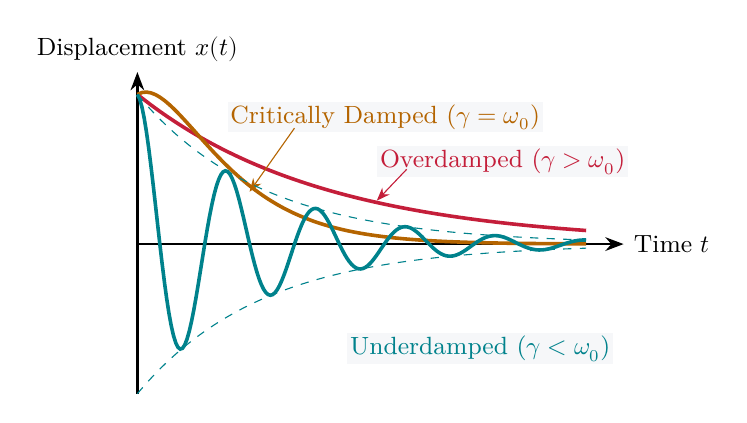
\begin{tikzpicture}[scale=0.95]
  % Axes
  \draw[-Stealth, thick] (0,0) -- (6.5,0) node[right] {\small Time $t$};
  \draw[-Stealth, thick] (0,-2) -- (0,2.3) node[above] {\small Displacement $x(t)$};
  
  % Overdamped curve
  \draw[myred, line width=1.3pt, domain=0:6, samples=100] plot (\x, {2.0*exp(-0.4*\x)});
  \node[myred, fill=mygray, inner sep=1pt, anchor=west] at (3.2, 1.1) {\small Overdamped ($\gamma > \omega_0$)};
  \draw[-Stealth, thin, myred] (3.6, 1.0) -- (3.2, 0.58);
  
  % Critically damped curve
  \draw[myamber, line width=1.3pt, domain=0:6, samples=100] plot (\x, {2.0*(1+1.8*\x)*exp(-1.5*\x)});
  \node[myamber, fill=mygray, inner sep=1pt, anchor=west] at (1.2, 1.7) {\small Critically Damped ($\gamma = \omega_0$)};
  \draw[-Stealth, thin, myamber] (2.1, 1.55) -- (1.5, 0.7);
  
  % Underdamped curve
  \draw[myteal, line width=1.3pt, domain=0:6, samples=200] plot (\x, {2.0*exp(-0.6*\x)*cos(360*\x/1.2)});
  \node[myteal, fill=mygray, inner sep=1pt, anchor=west] at (2.8, -1.4) {\small Underdamped ($\gamma < \omega_0$)};
  
  % Envelope
  \draw[dashed, myteal, thin, domain=0:6, samples=100] plot (\x, {2.0*exp(-0.6*\x)});
  \draw[dashed, myteal, thin, domain=0:6, samples=100] plot (\x, {-2.0*exp(-0.6*\x)});
\end{tikzpicture}
\end{tcolorbox}

% =============================================================================
% QUICK REVISION PAGE
% =============================================================================
\newpage
\begin{center}
  {\large\bfseries\color{myred} Quick Revision --- Module 1}\\[3pt]
  {\small\color{mydark} Mechanics $|$ BS-PH101}
\end{center}
\noindent{\color{myred}\rule{\linewidth}{1.2pt}}
\vspace{4pt}

\begin{tcolorbox}[formulabox, title={\textbf{Key Formulas and Metrics at a Glance}}]
\renewcommand{\arraystretch}{1.35}
\begin{tabularx}{\linewidth}{B{5.0cm} X}
Degrees of Freedom & $f = 3N - k$ \quad ($N$ particles, $k$ constraints) \\[4pt]
Limiting Static Friction & $f_{s,\max} = \mu_s N$ \quad and \quad $\tan\lambda = \mu_s$ \\[4pt]
Potential Energy Relation & $\vec{F} = -\nabla V = -\left(\frac{\partial V}{\partial x}\hat{i} + \frac{\partial V}{\partial y}\hat{j} + \frac{\partial V}{\partial z}\hat{k}\right)$ \\[4pt]
Conservative Force Rule & $\nabla \times \vec{F} = 0 \iff \oint \vec{F} \cdot d\vec{r} = 0$ \\[4pt]
Coriolis Acceleration & $\vec{a}_{\text{cor}} = 2(\vec{\omega} \times \vec{v}')$ \quad (Deflection to right in Northern Hemisphere) \\[4pt]
Underdamped Frequency & $\omega_d = \sqrt{\omega_0^2 - \gamma^2}$ \quad ($\gamma = b/2m$) \\[4pt]
Quality Factor & $Q = \frac{\omega_0}{2\gamma} = \frac{\pi}{\delta} = \omega_0 \tau$ \\[4pt]
Resonance Amplitude Freq. & $\omega_r = \sqrt{\omega_0^2 - 2\gamma^2}$ \\[4pt]
Parallel Axis Theorem & $I = I_{\text{cm}} + M h^2$ \\[4pt]
Perpendicular Axis Theorem & $I_z = I_x + I_y$ \quad (Planar lamina in $xy$-plane) \\[4pt]
\end{tabularx}
\end{tcolorbox}

\begin{tcolorbox}[defbox, title={\textbf{One-Line Definitions}}]
\begin{itemize}[leftmargin=*, itemsep=2pt]
  \item \textbf{Holonomic Constraint:} A constraint expressible as an integrable algebraic equation of position coordinates and time $f(\vec{r}, t) = 0$.
  \item \textbf{Conservative Force:} A force field in which work done along any closed path is zero ($\oint \vec{F} \cdot d\vec{r} = 0$).
  \item \textbf{Coriolis Force:} A velocity-dependent fictitious force acting in a rotating reference frame ($\vec{F}_{\text{cor}} = -2m(\vec{\omega} \times \vec{v}')$).
  \item \textbf{Logarithmic Decrement:} The natural log of ratio of two consecutive amplitudes one period apart ($\delta = \gamma T_d$).
  \item \textbf{Radius of Gyration:} The perpendicular distance from axis of rotation where whole mass can be assumed concentrated ($I = M k^2$).
\end{itemize}
\end{tcolorbox}

\begin{tcolorbox}[exambox, title={\textbf{Frequently Asked / Viva Questions}}]
\begin{enumerate}[topsep=0pt, label=\textbf{Q\arabic*.}, itemsep=5pt]
  \item \Q{State the condition for a force field to be conservative.}
  A force field $\vec{F}$ is conservative if $\nabla \times \vec{F} = 0$ (irrotational) or equivalently work done around any closed loop $\oint \vec{F} \cdot d\vec{r} = 0$.

  \item \Q{Why is Coriolis force called a fictitious force?}
  Because it arises due to the acceleration of the observer's rotating frame of reference, not due to physical interactions between bodies.

  \item \Q{What is the physical significance of negative gradient of potential energy?}
  $\vec{F} = -\nabla V$ indicates force always points in direction of steepest decrease of potential energy towards stable equilibrium.

  \item \Q{Distinguish between holonomic and non-holonomic constraints with examples.}
  Holonomic constraints are integrable algebraic position relations (e.g. rigid body length); non-holonomic involve non-integrable velocity relations or inequalities (e.g. sphere rolling without slipping).

  \item \Q{What is critical damping and state its practical application?}
  Critical damping occurs when $\gamma = \omega_0$. The system returns to equilibrium in shortest time without oscillating. Used in car shock absorbers and deadbeat galvanometers.

  \item \Q{How does amplitude resonance frequency differ from velocity resonance frequency?}
  Amplitude resonance occurs at $\omega_r = \sqrt{\omega_0^2 - 2\gamma^2}$ while velocity resonance occurs exactly at natural frequency $\omega_v = \omega_0$.

  \item \Q{What is Quality Factor ($Q$) of an oscillator?}
  $Q = 2\pi \frac{\text{Energy stored}}{\text{Energy lost per cycle}} = \frac{\omega_0}{2\gamma}$. Higher $Q$ implies lower damping and sharper resonance.

  \item \Q{State Parallel and Perpendicular axes theorems of moment of inertia.}
  Parallel axis: $I = I_{\text{cm}} + Mh^2$. Perpendicular axis: $I_z = I_x + I_y$ for planar laminas.

  \item \Q{Why are track rails laid higher on outer curves?}
  To provide necessary centripetal force via component of normal reaction and eliminate reliance on lateral friction.

  \item \Q{Calculate the moment of inertia of a solid sphere of mass $M$ and radius $R$ about a tangent.}
  By parallel axis theorem, $I_{\text{tangent}} = I_{\text{cm}} + M R^2 = \frac{2}{5}M R^2 + M R^2 = \frac{7}{5}M R^2$.

  \item \Q{What is the total energy of a simple harmonic oscillator of mass $m$ and amplitude $A$?}
  $E = \frac{1}{2} m \omega_0^2 A^2$. Total mechanical energy is constant and continuously converts between kinetic and potential forms.

  \item \Q{Show that Coriolis force does no work on a moving particle.}
  $\vec{F}_{\text{cor}} = -2m(\vec{\omega} \times \vec{v}')$ is always perpendicular to velocity $\vec{v}'$. Power $P = \vec{F}_{\text{cor}} \cdot \vec{v}' = 0 \implies W = 0$.
\end{enumerate}
\end{tcolorbox}

\begin{tcolorbox}[tikzbox, title={Summary Comparison of Damped Motion Regimes}]
\centering
\begin{tabularx}{\linewidth}{|B{3.0cm}|Y|Y|Y|}
\hline
\textbf{Parameter} & \textbf{Overdamped ($\gamma > \omega_0$)} & \textbf{Critically Damped ($\gamma = \omega_0$)} & \textbf{Underdamped ($\gamma < \omega_0$)} \\
\hline
\textbf{Roots of Char. Eq.} & Real and distinct. & Real and equal ($r = -\gamma$). & Complex conjugate ($-\gamma \pm i\omega_d$). \\
\hline
\textbf{Motion Nature} & Non-oscillatory, slow return. & Non-oscillatory, fastest return. & Oscillatory with decaying amplitude. \\
\hline
\textbf{Frequency} & No frequency of oscillation. & No frequency of oscillation. & $\omega_d = \sqrt{\omega_0^2 - \gamma^2}$. \\
\hline
\textbf{Practical Use} & Heavy door closers. & Galvanometers, vehicle suspension. & Tuning circuits, musical strings. \\
\hline
\end{tabularx}
\end{tcolorbox}

\end{document}
